\documentclass[12pt]{article}
\usepackage[normalem]{ulem}
\usepackage{graphicx, multirow}
\usepackage{amsmath, array}
\usepackage{fancyheadings, lastpage}
\usepackage{pdflscape ,anyfontsize}
\usepackage{longtable}
\usepackage{listings}
\usepackage{algpseudocode}
\usepackage{changepage}
\usepackage[a4paper]{geometry}
\usepackage{pdfpages}
\renewcommand{\refname}{}
% REFERENCE http://tex.stackexchange.com/questions/4891/how-do-i-control-the-spacing-above-a-new-paragraph %
\makeatletter
\renewcommand{\paragraph}{
  \@startsection{paragraph}{4}
  {\z@}{3.25ex \@plus -10em \@minus 1em}{0.1em}
  {\normalfont\normalsize\bfseries}
}
\lstset{
    breaklines=true,
  }
\makeatother
\newcommand{\zeroindent}{\setlength{\parindent}{0pt}}
\setcounter{secnumdepth}{5}
\setcounter{tocdepth}{6}
\renewcommand{\headrulewidth}{0pt}
\lhead{Group Project 07 – Design Specification}
\rhead{(Release) -Version 2.9}
\lfoot{Aberystwyth University / Computer Science}
\cfoot{}
\rfoot{\thepage{}  of  \pageref{LastPage}}
\usepackage{graphicx}
\begin{document}
\pagestyle{fancy}
\begin{flushleft}
\rule[0.5cm]{13.8cm}{0.02cm}
\end{flushleft}
{\fontsize{20}{20}\selectfont \textbf {\centerline{Group Project 07 Design Specification}}}
\begin{flushleft}
\rule[0.5cm]{13.8cm}{0.01cm}
\end{flushleft}

\begin{tabular}{ l l }

\\ \multirow{1}{*}{\textit{Authors: }} & Mosopefoluwa David Adejumo \\  & Ryan Gouldsmith \\
& Harry Flynn Buckley \\ & Zack Lott \\ & Mark Radcliffe Pitman \\ & Jack Alexander Reeve \\ & Mark Alexander Smith \\ &Martin Vasilev Zokov \\ & Maciej Wojciech Dobrzanski \\
\\ \multirow{1}{*}{\textit{Config ref: }} & SE\_07\_DS\_01 \\
\\ \multirow{1}{*}{\textit{Date} } & \today \\
\\ \multirow{1}{*}{\textit{Version}} & 2.9 \\ 
\\ \multirow{1}{*}{\textit{Status}} & Release \\

\end{tabular}


\vspace{3.2cm}
\hfill\begin{minipage}{\dimexpr\textwidth-0.3cm}
Department of Computer Science \\
Aberystwyth University \\
Aberystwyth \\
Ceredigion\\
SY23 3DB \\
Copyright \small{\copyright}\\ Aberystwyth University 2013
\end{minipage}


\newpage
\tableofcontents{}
\newpage
\section{INTRODUCTION}
\subsection{Purpose}
The purpose of this document is to, specify the technical design of both the Android and web applications. It will go into detail regarding functions. This will allow us to more easily designate tasks to team members when it comes to coding week. It will also show how these functions interact with each other and how the website, server and Android app interact through the use of sequence diagrams. The document is structured in a way that makes it easy to refer to when the programmer needs clarification on how to build a certain function. The document will also show how the database will be structured and what the field names will be.
\subsection{Scope}
This document, will cover all aspects of the Android and web design and their implementation. It should be read by all members of the group and approved by the client. It will be used as a guide for the programmers to build from in coding week. The document will allow the team leader to assign a given function to a team member which they can then code.
\subsection{Objective}
The precise areas which this document will cover are:
\begin{itemize}
\item Provide a clear class diagram, covering all aspects of the Android app.
\item Define, in detail, the interaction between all the programs in the system.
\item Provide a structure for implementation of the applications.
\item Outline the significant systems to be used in the applications.
\item Provide descriptions of functions.
\end{itemize}
\newpage
\section{ARCHITECTUAL DESCRIPTION}
\subsection{Programs In System}
The walk tour application consists of:
\begin{itemize}
\item The Android application. 
\item The Data server. 
\item The Website application.
\end{itemize}
\subsubsection{The Android Application}
\par{The Android application is used to create physical data representing a route allowing the users to record and upload a walk. It allows the user to add points of interest along a route and associate images. It displays a map screen and is used to record location data for a walk using GPS. It also gives the user options to add pictures to a walk. \newline Requirements Covered: (FR1, FR2, FR3, FR4, FR5, FR6, FR7,FR9, EIR1, PR1)}
\subsubsection{The Database Server}
Stores walk info in MySQL which it receives from the Android application as a MIME type. When the server application receives information for a walk it appends the location data to the database and stores all pictures on the server machine. The database server will also have a PHP file which handles the uploading of data from the Android device. The file that handles the upload can be accessed via the URL in a browser, but doing so will present an error message.
Requirements Covered: (DC3)
\begin{itemize}
	\item List of Walks relation:
	\begin{itemize}
		\item id
		\item title
		\item shortDesc
		\item longDesc
		\item hours
		\item distance
	\end {itemize}
	\item Location
	\begin{itemize}
		\item id
		\item walkID
		\item latitude
		\item longitude
		\item timestamp
	\end{itemize}
	\item Place description
	\begin{itemize}
		\item id
		\item locationId
		\item name
		\item description
	\end{itemize}
	\item Photo Usage
	\begin{itemize}
		\item id
		\item placeId
		\item photoName
	\end{itemize}
\end{itemize}
\subsubsection{Web Application}
Allows the user to view walks in more detail. The website is also hosted on the data server and can be used for viewing information about walks including route taken, points of interest and pictures. This program overlaps with 1.1.2 (Database Server). It interacts with the database using PHP. 
Requirements covered: (FR8, FR9)
\subsection{Significant Classes}
\subsubsection{Android Application}
This section describes the most significant classes in the application. The complete set of classes can be seen in the class diagram – Section 4.1.2. These classes will all be written in Java.
\paragraph{WalkModel}
\zeroindent
A WalkModel holds all the data concerning a single route, this includes a list of all location points that trace the path and a list of all the places of interest.
\paragraph{RouteRecorder}
\zeroindent
The RouteRecorder retrieves the current location from the system, and depending on factors such as speed and direction, the location information will be added to the local WalkModel. This class will carry out some analysis of the path traveled so far to determine when to record points,i.e. if a recorded path seems to be traveling in a straight line then fewer point will be need added than if the path traces a circle.
\paragraph{FileTransferManager}
\zeroindent 
A connection will be made with the server via the FileTransferManager. It is responsible uploading and downloading WalkModels, including all associated images, from the database server. This class only interacts with the WalkManager, so any objects wishing to upload of download content must connect through WalkManager, this is to add an extra layer of abstraction that simplifies the solution.
\paragraph{WalkScreen}
\zeroindent
This is the main class, which creates the RouteRecorder. All the data handling for a walk is completed in this Activity. The method for image handling are also called within this class as well as the pop-ups; these are created within the same activity. Adding the points of interest along a walk are also used in this Activity. The uploading a walk will also be called from this Activity too.
\subsubsection{Database Server}
The files here are used to control the interaction between the database and the other programs in the module. All these files will be written in PHP. Object Oriented Programming will not be implemented in this system.
\subsubsection{Web Application}
The following are files in PHP that will be used to interact between the database and the website. These are also pages that will be visible and accessible by the user unless otherwise stated. Object Oriented Programming will not be implemented in this system.
\paragraph{Index}
This file will serve as the homepage and holds links to view the list of walks and terms of service.
\paragraph{Walk List}
This file will process information from our database and display it as a list of walks.
The walks will be clickable in order to view them in more detail. Users will be able to select a walk via this file
\paragraph{Walk Details}
This file will be used to give the user a more in depth look at a specific walk.
This means they will be able to see a map view, images taken on the walk, and points of interest.
\paragraph{Google Maps Api}
The Google Maps API will be used to portray a persons walk data into a visual map.
The user will also be able to view points of interest on the map. This will serve as a separate file that will interact with Google’s system.
\paragraph{File\_Saver}
The Apache HTTP Client will be used for by the android application to send data to our database server. This will mean our application will be able to 'POST' data to the server. This reduces load on the server compared to our previous idea of zipping and unzipping each set of files for a walk. The data will be sent as a JSON string. This file will decode the JSON string and add all the walk data to the appropriate tables where required
\subsection{Table Mapping Requirements Onto Classes}
This section gives an overview of what classes/files cover what requirements as specified by the client.

\begin{tabular}{|p{1cm}|p{10cm}|}
\hline
	FR1 & WalkScreen, WalkSetupScreen, MainMenuScreen, CancelWallkView\\
\hline
	FR2 & WalkScreen, RouteRecorder, WalkModel\\
\hline
	FR3 & LocationPoint, PointOfInterest\\
\hline
	FR4 & LocationPoint, PointOfInterest\\
\hline
	FR5 & CancelWalkView, EditWalkView\\
\hline
	FR6 & WalkManager, FileTransferManager
\\
\hline
	FR7 & RouteRecorder\\
\hline
\end{tabular}
\newpage
\section{DEPENDENCY DESCRIPTIONS}
\subsection{Component Diagrams}
\subsubsection{Android}
\begin{figure}[htp]
\centering
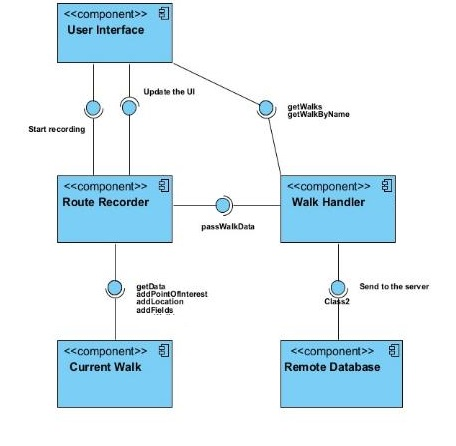
\includegraphics[scale=0.90]{Design/AndroidDP.jpg}
\caption{Android Dependency Diagram}
\label{Android Dependency Diagram}
\end{figure}

\subsubsection{Website}
\clearpage
\begin{figure}[htp]

\centering
\includegraphics[scale=0.50]{Design/web_diagram.png}
\caption{Web Component Diagram}
\label{Web Component Diagram}
\end{figure}
\subsubsection{Database Server}
\section{INTERFACE DESCRIPTION}
This section contains method and class declarations for all major aspects of the program. The following code describes sthe public methods that are used in the program.
\subsection{Screens}
The following classes all extend Activity and are used to control the display.

\subsubsection{MainMenuScreen}
\begin{lstlisting}[language=java]
/**
 * This class is responsible for displaying the main menu 
 * screen, and reacting
 * to button presses. It is the first screen that is 
 * presented to the user.
 * /
public class MainMenu extends Activity{

/**
 * Starts a new WalkSetupScreen activity, and displays it
 * to the user. It is
 * called when the user presses the start walk button.
 * @param v is the View that is called the method.
 */
public void startWalkSetupScreen(View v);
}
\end{lstlisting}
\subsubsection{WalkSetupScreen}
\begin{lstlisting}[language=java]
/**
 * This class is responsible for displaying the walk setup
 * screen which sets the
 * title and descriptions for a walk
 */
public class WalkSetupScreen  extends Activity{

   /**
    * Starts a new WalkScreen activity, displays it to the 
    * user and starts
    * recording GPS data. The details that the user has 
    * input, are passed to the
    * new activity.
    * @param v  is the View that called this method
    */
   public void startWalk(View v) ;
}
\end{lstlisting}
\subsubsection{WalkScreen}
\begin{lstlisting}[language=java]
/**
 * This class is responsible for displaying the walk screen
 * and reacting to button presses.
 */
public class WalkScreen extends extends Activity {

   /**
    * creates and displays a AddPoiView.
    * @param v , is the object that called the method.
    * @param v, is the object that called the method.
    */
   public void addPOI(View v);

   /**
    * creates and displays a WalkFinishedView.
    * @param v, is the object that called the method.
    */
   public void finishWalk(View v);

   /**
    * creates and displays a EditWalkView.
    * @param v, is the object that called the method.
    */
   public void editWalkDialog(View v);

   /**
    * creates and displays a CancelWalkView.
    * @param v, is the object that called the method.
    */
   public void cancelWalk(View v);

   /** 
    *Opens the gallery to add a picture to the current walk
    * @param v the object that called the method
    */
   public void getFromGallery(View v);

   /** Opens the camera app to take a picture that will be
    * added to the walk.
    * @param v the object that called the method
    */
   public void getFromCamera(View v);

   /** Adds a new point of interest*/
   public void addPoi();

   /** Starts the upload of a walk to the server.*/
   public void uploadWalk();

   /**
    * returns the user to the start screen, is called 
    * either after the upload has
    * finished or when the user cancels the walk.
    * @param status, 
    * */
   public void returnToStart(boolean status);
}
\end{lstlisting}
\subsection{Views}
Views are subsections of the screen. Here we use popup windows to both inform the user and prompt user input.
\subsubsection{DialogView}
\begin{lstlisting}[language=java]
/**
 * An abstract class to easily create different 
 * popup screens which can be
 * customzied. Implements the OnClickListener interface to 
 * repsond to key
 * presses.
 */
public abstract class DialogView implements OnClickListener {
   /** Destroys the popup */
   public void dismiss();

   /** Displays the popup */
   public void show() ;
}
\end{lstlisting}
\subsection{Models}
The model classes are used to store the walk data
\subsubsection{WalkModel}
\begin{lstlisting}[language=java]
/**
 * stores all information about a single walk
 */
public class WalkModel {    

   /**
    *  @return the name of the walk.
    */
   public String getTitle();

   /**
    * Sets the name of the walk
    * 
    * @param the new name of the walk.
    * 
    */
   public void setTitle(String newTitle);

   /**
    *  @return a short description of the walk 
    */
   public String getShortDescription() ;

   /**
    * @param newShortDesc,set the short description of the
    * walk. 
    */
   public void setShortDescription(String newShortDesc) ;

   /** 
    * @return a long description of the walk.
    */
   public String getLongDescription();

   /**
    *  @param newShortDesc,set the long description for the walk.
    */
   public void setLongDescription(String newLongDesc);

   /**
    * @return a vector of all the LocationPoint in the walk. 
    * Including PointsOfInterests
    */
   public Vector<LocationPoint> getRoutePath();

   /** 
    * adds a LocationPoint to the walk. 
    * 
    * @param point, the location you want to add
    */
   public void addLocation(LocationPoint point);

   /**
    * works out the total distance traveled along the walk.
    * 
    * @return the running total of km traveled. 
    */
   public double getDistance();
   /** 
    * works out the total time taken.
    * 
    * @return the elapsed time since the walk was started
    */
   public double getTimeTaken();


}
\end{lstlisting}
\subsubsection{LocationPoint}
\begin{lstlisting}[language=java]
/**
 * This class stores a map position and records the time at 
 * which is was taken
 * /
public class LocationPoint {
/**
 * @return the Time that the recording was made
 */
public long getTime();   

/**
 * @return the longitude, the east/west distance from 
 * Greenwich.
 */
public double getLongitude();

/**
 * @return the latitude, the north/south distance from the equator.
 */
public double getLatitude();

/**
 * works out the distance between two locations.
 * 
 * @param point is the first location
 * @param point1 is the second location
 * @return the distance between the two locations in 
 * kilometers
 */
public static double distBetween(LocationPoint point, LocationPoint point2);
}
\end{lstlisting}
\subsubsection{PointOfInterest}
\begin{lstlisting}[language=java]
/**
 * Stores information about a place of interest
 */
public class PointOfInterest extends LocationPoint{

   /**
    * adds reference to an image to the poi.
    * 
    * @param newImage,is the image that is to be added
    */
   public void addImage(ImageInformation newImage);

   /**
    *  @return all the images associated with this point. 
    */
   public Vector<ImageInformation> getImages();

   /** 
    * @return the description of this place. 
    */
   public String getDescription();

   /** 
    * @param desc, sets the description of this point.
    */
   public void setDescription(String desc);

   /**
    * gets the title of the POI
    * 
    * @return String the title of the walk
    */
   public String getTitle();

   /** sets the title of this point.
    * 
    * @param title, new title
    */
   public void setTitle(String title);


}

\end{lstlisting}
\subsection{Controllers}
Below are the important classes that interact with the walk model.
\subsubsection{RouteRecorder}
\begin{lstlisting}[language=java]
public class RouteRecorder extends Service implements LocationListener{
   /**
   	* Gets the last known position
    * @return LocationPoint object
    * 
    */
   public LocationPoint getLastKnownPosition();

   /**
    * saves the location in the WalkModel object
    * 
    * @param loc
    */
   public void newLocation(LocationPoint loc);

   /**
    * stops the recoding of locations.
    */
   public void finishWalk();
}
\end{lstlisting}
\subsubsection{FileTransferManager}
\begin{lstlisting}[language=java]
/**
 * Handles the encoding and uploading of walk data.
 */
public class FileTransferManager{

   /**
    * makes a connection to data server and uploads all 
    * files belonging to the
    * given file.the return value will be zero if the 
    * method succeeded without problems.
    * @param walk,the walkModel that will be sent to the 
    * server
    */
   public int uploadWalk(WalkModel walk);
}
\end{lstlisting}
\section{DETAILED DESIGN}
This section details the algorithms and interactions that will be implemented in the program. The algorithms used may differ from the final product.
\subsection{UML Diagrams}
\subsubsection{Android Sequence Diagram}\clearpage
\begin{figure}[htp]

\begin{adjustwidth}{-3cm}{0cm}
\centering
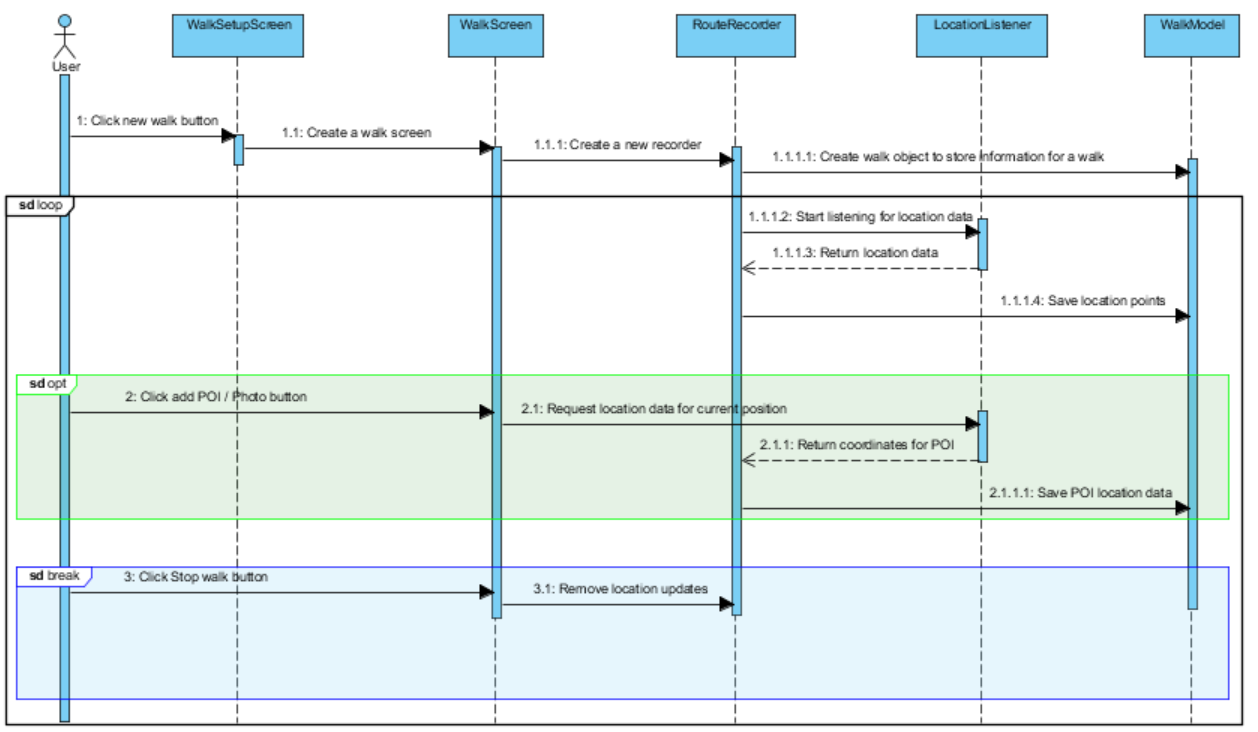
\includegraphics[scale=0.90]{Design/route_record_sequence_diagram.PNG}
\caption{Android Sequence Diagram}
\label{Android Sequence Diagram}
\end{adjustwidth}
\end{figure}
The sequence diagram describes the recording of a walk and how the classes which are involved in the process interact.
In action 1. the user is prompted for details in the WalkSetupScreen and after he/she presses the start walk button, a map screen is shown and a RouteRecorder and WalkModel objects are created. After that the application goes into a loop of actions from the RouteRecorder, LocationListener and WalkModel classes. The recorder asks the listener for location data and when the data is returned, it is saved in the WalkModel's array of location points.
Action 2 is optional for the user, because it is not mandatory to have a Point of interest or photos in every walk. If a user decides to click the “Add POI” button, the LocationListener gives the coordinates of the current location to the RouteRecorder and they are saved in the WalkModel object.
Action 3 is the exit point of the loop for the current walk recording. It is done by clicking the stop button which brakes the loop.
The LocationListener is deliberately not activated at all times while a walk is in progress in order to save battery life.
\subsubsection{Sequence Diagram For Web}
\begin{figure}[htp]
\begin{adjustwidth}{-2cm}{0cm}
\centering
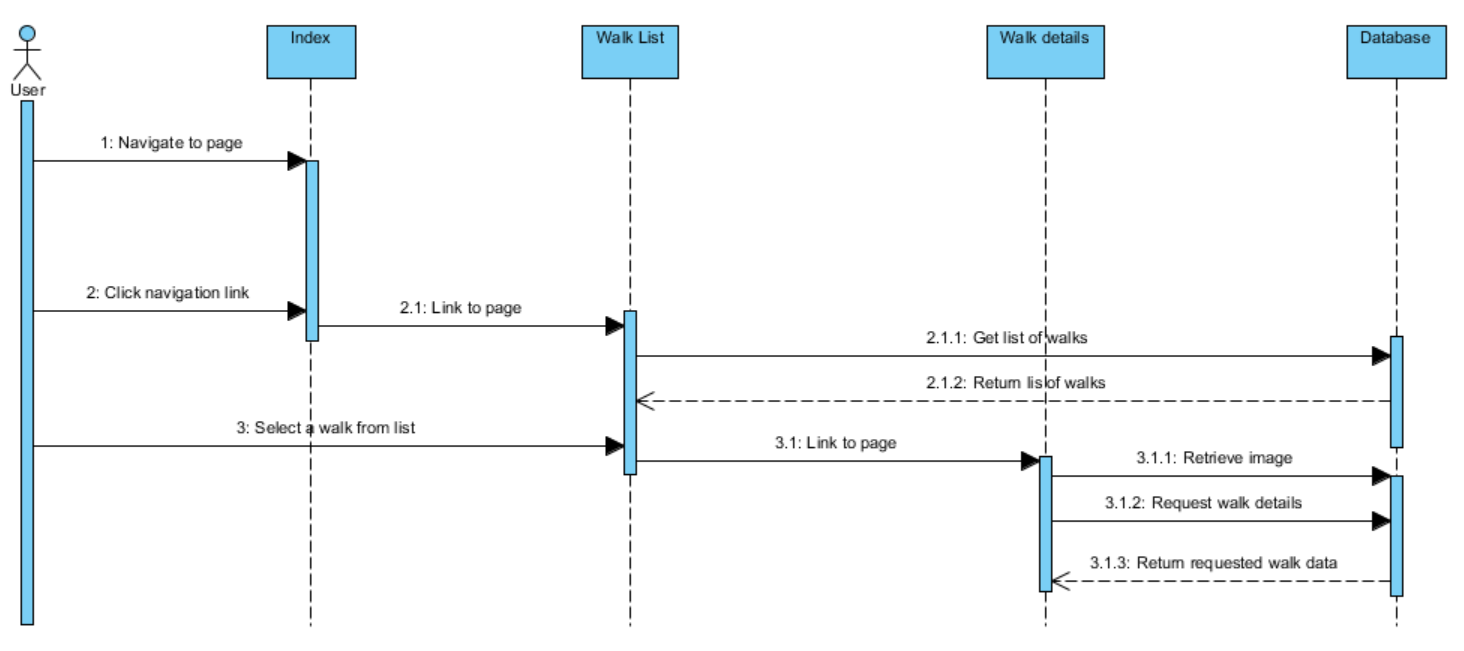
\includegraphics[scale=0.70]{Design/web_sequence_diagram.PNG}
\caption{Web Sequence Diagram}
\label{Web Sequence Diagram}
\end{adjustwidth}
\end{figure}
The sequence diagram describes the user interaction with the website, and the websites interaction with the database.
In action 1, the user navigates to the index page either via a link or via the URL
In action 2, the user navigates to a page where a list of walks is displayed. The list shows all the information in the database at any one given time.The only information gathered from the database will be the walks location, title, short description and thumbnail image if possible.
In action 3 the user can view a selected walk. The file will fetch in addition to the data fetched in action 2, the long description, all images associated with the walk, the duration of the walk and all the points of interest. The user can then click on a point of interest for further information about a walks location.
Both the walk details and the walk list page can link back to the index page. All pages can easily be accessed via the URL however, if the user attempts to visit the walk details page via the URL, they will be redirected to the walk list page and given an error message.
\clearpage
\subsubsection{Overall Interaction Sequence Diagram}

\begin{figure}[htp]
\begin{adjustwidth}{-2cm}{0cm}
\centering
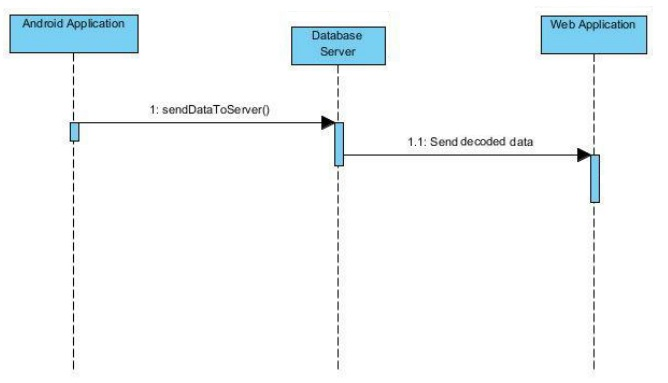
\includegraphics[scale=0.80]{Design/sequence_diagram.jpg}
\caption{Overall Sequence Diagram}
\label{Overall Sequence Diagram}
\end{adjustwidth}
\end{figure}
This diagram details the sequence in which data is sent and retrieved and how the Web Application and Android Applications interact with the database. Not all these interactions may be completed in one sitting. The Android application and Web Application interact independently of each other. In action 1 the Android Application gathers all the information about a walk including images and sends it to the HTTP Protocol via a post request in the form of a JSON file. In action 2 the HTTP Protocol, via the Apache HTTP Client, encodes the data for sending to the database, this is done via a JSON file as a MIME type, the image is encoded as a based 64 string. In action 3 The Data Layer decodes the JSON from the Android and stores it in the database. On request theData Layer retrieves the data from the database and sends it to the Web Application. In action 4 The Web Application requests information that is retrieved from the database. In the event that such information is not found, the Web Application displays an error to the user.

\subsection{Class Diagram}
\newgeometry{top=1.5cm, bottom =-0.8cm}
\begin{landscape}
\begin{adjustwidth}{0.5cm}{2cm}
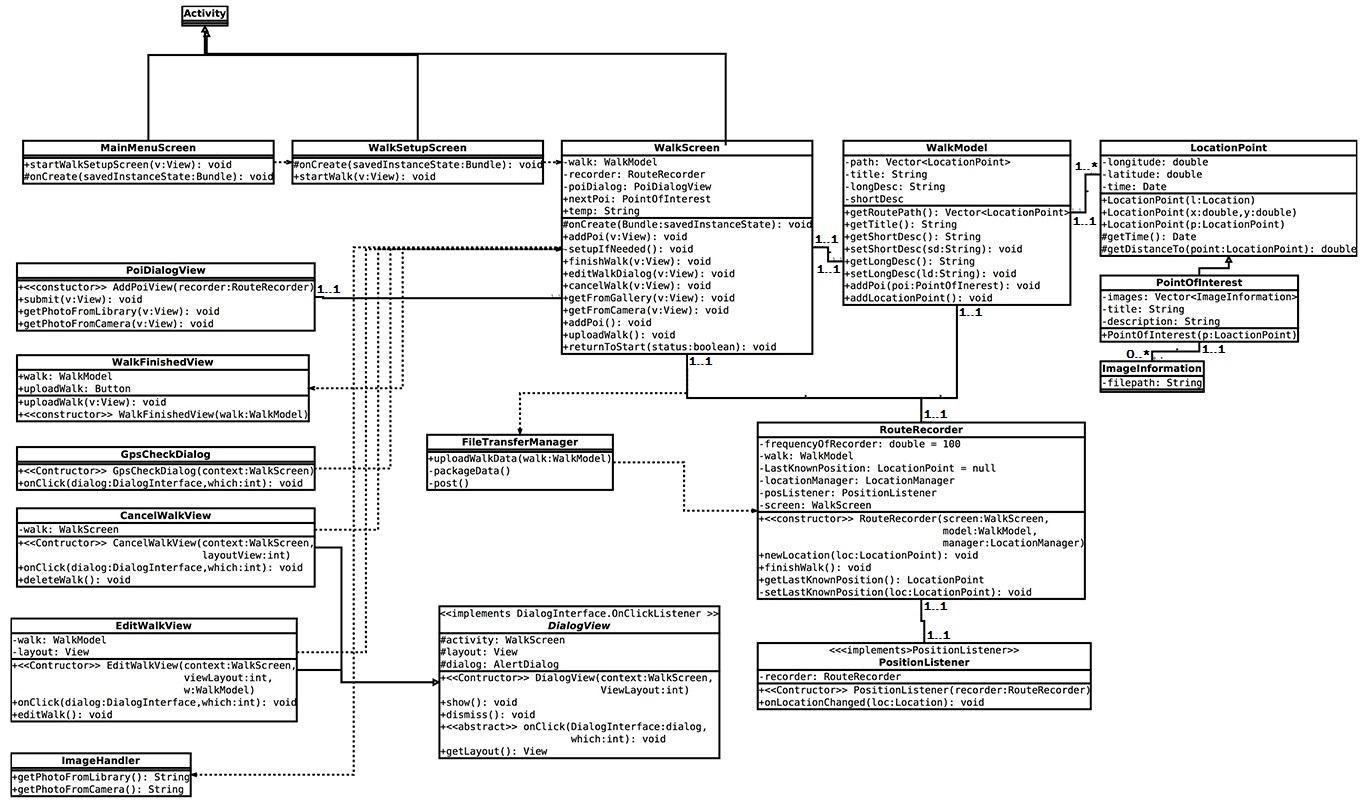
\includegraphics[scale=2.74253]{Design/class_diagram_new.jpg}
\end{adjustwidth}
\end{landscape}
\restoregeometry
The classes ending in ‘screen’, are all Activities. They all, in some way, display a layout to the screen and respond to user input. Any response that requires further processing would be passed to another class and then handed back to be displayed, but it would be the ’screen’ class itself that initialised the action.  
There are several classes that have been suffixed with ‘View’, these classes all extend the android class View. They are all visible to the user and act much like ‘screen’ classes except that they don’t use the whole screen and do not change the displayed screen only create new Views.  
The classes WalkModel,PointOfInterest and LocationPoint can all be considered to be model classes. They are used to store the walks data in an organised fashion, and have no methods to do anything other than to set and get information.  
WalkManager, ImageHandler and FileTransferManager all perform some tasks that are not immediately apparent to the user. They are the utility classes that are used by others.
\subsection{Significant Algorithms}
\subsubsection{Android Algorithms}
\paragraph{RouteRecorder Algorithm}
\zeroindent
\begin{algorithmic}
\While{walk not finished}
	\State get location
	\If{distance between new location, old location than X}
		\State add new location to walkModel
	\EndIf
\EndWhile
\end{algorithmic}
\paragraph{JSON Encoder}
\begin{algorithmic}
\State json.add("title", data.getTitle )
\State json.add("short\_desc", data.getShortDescription )
\State json.add("long\_desc", data.getLongDescription )
\State json.add("hours", data.getTimeTaken )
\State json.add("distance", data.getDistance )

\For{ all data getPath as point}
   \State locationObject.add("longitude", point.getLongitude )
   \State locationObject.add("latitude", point.getLatitude )
   \State locationObject.add("time", point.getTime )
   \If{point is an instance of PointOfInterest}
      \State locationObject.add("description",point.getDescription )
      \State locationObject.add("title", point.getTitle )
      \For{all point.getImages  as image}
         \State imagObject.add ("file\_data", image.getImageAsString )
         \State imageArray.add imagObject
      	\State location.put("images", images)
      \EndFor
   \EndIf
  \State pointsArray.put(locationObject)
\EndFor
\State json.add("route", pointsArray)
\end{algorithmic}
\subsubsection{PHP Algorithms}
\paragraph{Connect To The Database}
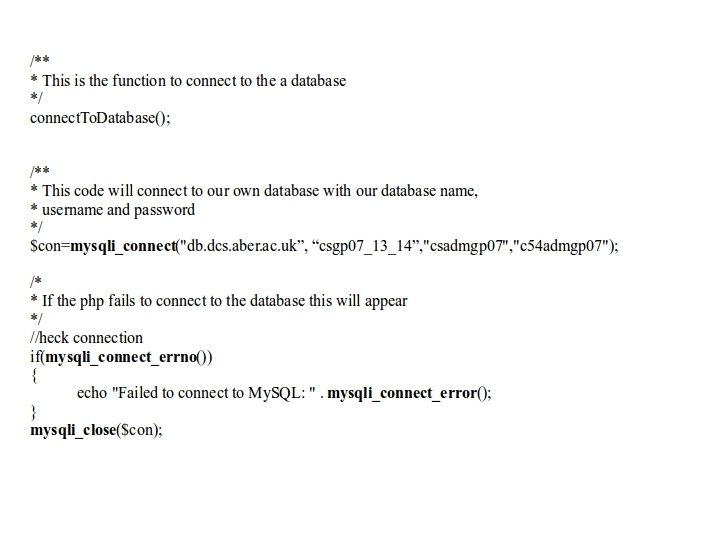
\includegraphics[scale=0.8]{Design/phpcode.jpg}
\paragraph{Append To The Server Database}
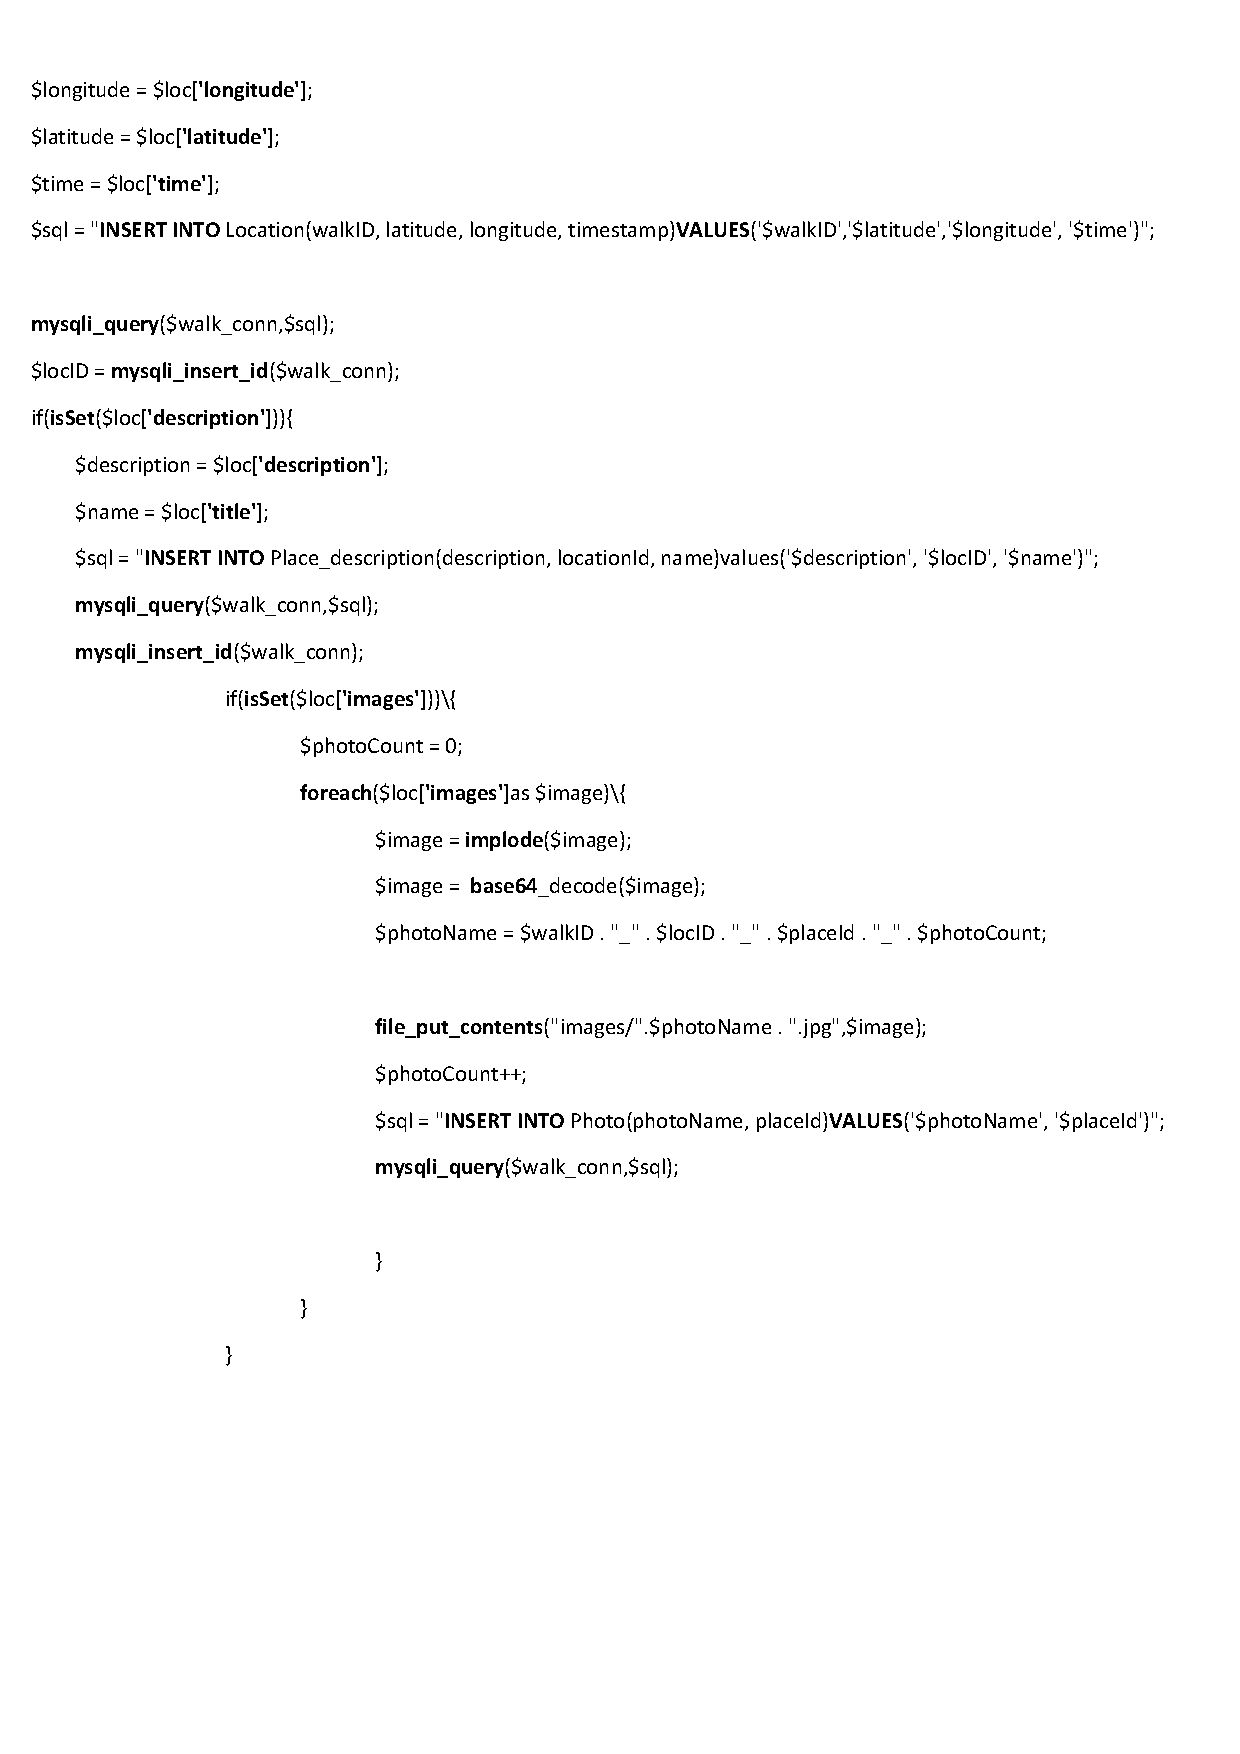
\includepdf[pages=-, pagecommand={}, scale=0.8]{Design/php.pdf}
\subsection{Significant Data Structures}
\subsubsection{WalkModel}
This is the most significant data structure in the Android application. It contains the information for the route taken,
all of the GPS coordinates that the user has walked through, Points of interest.
\subsubsection{LocationPoint}
This class is responsible for storing a point on the map. It has variables for longitude, latitude and a timestamp.
After a GPS reading is taken for the current physical location is taken, it is put in an object
of this class and stored in the WalkModel.
\subsubsection{PointOfInterest}
This data structure is used when adding a point of interest. It holds information for the description and title of a POI.
The class extends the LocationPoint so a POI can have location coordinates and a time
stamp.
This data structure is used when adding a point of interest. It holds information for the description and title of a POI.
The class extends the LocationPoint so a POI can have location coordinates and a time
stamp.
\newpage 
\section{REFERENCES}
\begin{thebibliography}{0}
\bibitem{Requirements1.2}
  Software Enginerring Group Projects
  \emph{Requirements Specification}.
   C. J. Price and B.P.Tiddeman, 
   1.2 (Release), 
   7 November 2013
\bibitem{DesignStand 1.6}
Software Engineering Group Projects. 
\emph{Design Specification Standards}.
	C. J. Price and N. W. Hardy, 
	SE.QA.05A,
	1.6. Release.
\bibitem{ProjectPlan1.8}
Software Engineering Group Projects
\emph{ Project Plan}.
Mosopefoluwa David Adejumo, R. Gouldsmith and others 1.8
(Release). 6th November 2013
\end{thebibliography}
\newpage

\section{DOCUMENT HISTORY}
\setlength\LTleft{-0.5cm}
\begin{longtable}{|p{1.3cm}|p{1.5cm}|p{2cm}|p{7cm}| p{2cm}|}
\hline
	Version & CFF No. & Date & Section Changed From Previous Version & Changed by \\
\hline
	1.0 & N/A & 28/11/13 & Created original document & HFB1 \\ 
\hline
	1.1 & N/A & 01/12/13 & Added sections created by other members. 
Updated config reference 
Updated layout. & MDA
 \\
\hline
	1.2 & N/A & 01/12/13 & Fixed some formatting issues, added information to what fields will be used. & RYG1 \\
\hline 
	1.3 & N/A & 04/12/13 & Added a new sequence diagram and a description for section 1.2 & MVZ
\\
\hline 
	1.4 & N/A & 05/12/13 & Updated section 1.1. Added descriptions to all sections & MDA \\
\hline 
	1.5 & N/A & 05/12/13 & Added a sequence diagram for the web.
 & MRP2 \\
\hline
	1.6 & N/A & 05/12/13 & Updated class diagram, added FileTransferManager interface. & HFB1 \\
\hline 
	1.7 & N/A & 06/12/13 & Added Apache HTTP Client description. & JAR39 \\
\hline 
	1.8 & N/A & 06/12/13 & Added methods to the MapView interface. & HFB1
 \\
\hline	
	1.9 &N/A&06/12/13&Changed sequence diagram for web and added
overall interaction sequence diagram & MVZ\\
\hline 
	2.0&N/A&06/12/13&Updated the Introduction section.&JAR39,
MRP2 \\
\hline
	2.1&N/A&06/12/13&Added web app diagram and Significant algorithms &ZAL \\
\hline 
	2.2&N/A&06/12/13&Updated author list. Updated formatting. Merged different versions of the document&MDA\\
\hline
	2.3&N/A&06/12/13& Added image reference numbers. Updated images 
from MWD5 and MAS69. Added missing images. Added images and descriptions to section 3.Added references. & MDA\\
\hline 
	2.4&N/A&06/12/13&Formatting corrections. Changed version&MDA \\
\hline 
	2.5&N/A&12/02/14&Re-wrote in LaTeX, removing feature creep &RYG1 \\
\hline
	2.6&N/A&13/02/14&Minor error checks and removal &MDA \\
 \hline
 	2.7&N/A&13/02/14&Added Images & RYG1\\
 \hline
 2.8&N/A&13/02/14&Added Sequence Diagrams &RYG1\\
 \hline
 2.9&N/A&13/02/14&Updated database file saver algorithm &MDA\\
 \hline
\end{longtable}

\end{document}